\documentclass[tikz,border=2pt]{standalone}
\usepackage{amsmath}
\usepackage{pgfplots}
\pgfplotsset{compat=1.18}

\begin{document}
% The optimal value V(b) as a function of the constraint level b: its slope at b_0 is the
% shadow price, the Lagrange multiplier of that constraint, i.e. the marginal value of one
% more unit of the resource.
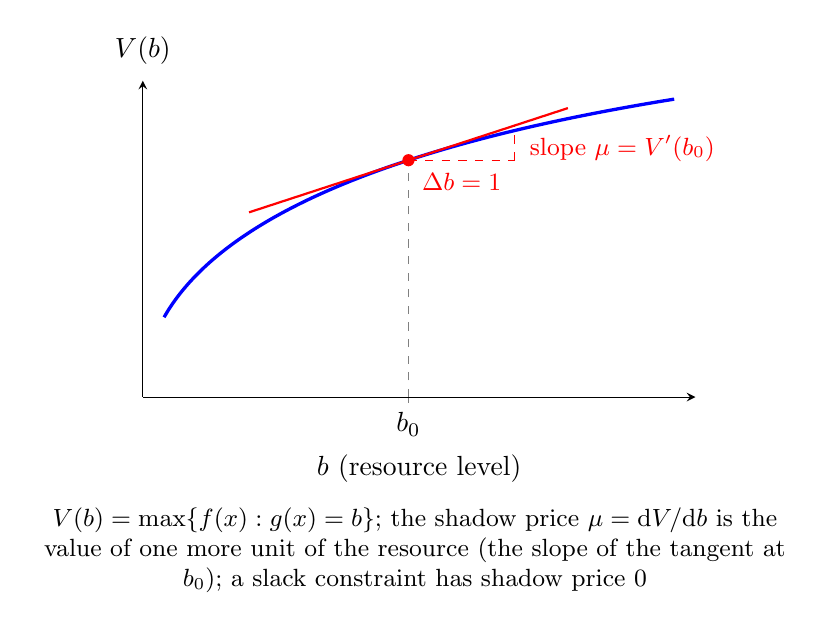
\begin{tikzpicture}
	\begin{axis}[
		axis lines=left, xmin=0, xmax=5.2, ymin=0, ymax=5.0,
		xtick={2.5}, xticklabels={$b_0$}, ytick=\empty,
		xlabel={$b$ (resource level)}, ylabel={$V(b)$}, ylabel style={rotate=-90, anchor=south, at={(axis description cs:0,1.02)}},
		samples=120, smooth, width=8.6cm, height=5.6cm, clip=false
		]
		\addplot[blue, very thick, domain=0.2:5] {3*sqrt(x)-0.4*x};
		\addplot[red, thick, domain=1.0:4.0] {3.743+0.549*(x-2.5)};
		\draw[gray, dashed] (axis cs:2.5,0) -- (axis cs:2.5,3.743);
		\draw[red, dashed] (axis cs:3.5,3.743) -- (axis cs:3.5,4.292);
		\draw[red, dashed] (axis cs:2.5,3.743) -- (axis cs:3.5,3.743);
		\fill[red] (axis cs:2.5,3.743) circle (2.2pt);
		\node[red, font=\small, anchor=west] at (axis cs:3.55,3.93) {slope $\mu=V'(b_0)$};
		\node[red, font=\small, anchor=north] at (axis cs:3.0,3.7) {$\Delta b=1$};
	\end{axis}
	\node[anchor=north, font=\small, align=flush center, text width=9.6cm] at ([yshift=-2pt]current axis.outer south) {$V(b)=\max\{f(x): g(x)=b\}$; the shadow price $\mu=\mathrm dV/\mathrm db$ is the value of one more unit of the resource (the slope of the tangent at $b_0$); a slack constraint has shadow price $0$};
\end{tikzpicture}
\end{document}
